\section{基于知识激活的少样本微调}

使用特定任务提示对预训练语言模型进行微调,已成为文本分类中一种很有前景的方法。特别地,以往研究表明,在数据量少的场景下,提示微调相较于使用额外分类器的通用微调方法具有显著优势。提示微调的核心思想是在输入中插入文本片段,即模板,并将分类问题转化为掩码语言建模问题,其中关键一步是在标签空间和标签词空间之间构建一个投影,即语言表达器(verbalizer)。语言表达器通常是手工制作的,或者通过梯度下降搜索得到,这可能会导致覆盖范围不足,并给结果带来相当大的偏差和高方差。在这项工作中,我们专注于将外部知识融入语言表达器,形成一种\textbf{知识型提示微调}(KPT),以改进并稳定提示微调。 

\subsection{方法设计}

\subsubsection{提示微调概述}
设 ${\mathcal{M}}$ 为在大规模语料库上预训练的语言模型。

在文本分类任务中,输入序列 $\mathbf{x} = (x_0,x_1,...,x_n)$ 被分类为类别标签 $y\in \mathcal{Y}$。提示微调将分类任务形式化为掩码语言建模问题。具体来说,提示微调将输入序列包裹在一个\emph{模板}中,模板是一段自然语言文本。

例如,假设需要将句子 $\mathbf{x}$ =“速度与加速度之间的关系是什么?”分类为标签 \textsc{科学}(标记为1)或 \textsc{体育}(标记为2),本文将其包裹为

\begin{equation*}
    \mathbf{x}_{\text{p}}=\text{\texttt{[CLS]} 一个 \texttt{[MASK]} 问题:} \mathbf{x}
\end{equation*}
然后 ${\mathcal{M}}$ 给出词汇表中每个词 $v$ 填入 \texttt{[MASK]} 标记的概率 $P_{\mathcal{M}}(\texttt{[MASK]}=v|\mathbf{x}_{\text{p}})$。
为了将词汇的概率映射到标签的概率,本文定义了一个\emph{语言表达器},即从词汇表中的少量词(构成\emph{标签词}集 $\mathcal{V}$)到标签空间 $\mathcal{Y}$ 的映射 $f$,即 $f\colon \mathcal{V} \mapsto \mathcal{Y}$。本文用 $\mathcal{V}_y$ 表示映射到特定标签 $y$ 的 $\mathcal{V}$ 子集,$\cup_{y\in\mathcal{Y}} \mathcal{V}_y = \mathcal{V}$。然后标签 $y$ 的概率 $P(y|\mathbf{x}_{\text{p}})$ 计算为


\begin{equation}
   P(y|\mathbf{x}_{\text{p}}) \!\!=\!\! g\left(P_{\mathcal{M}}(\texttt{[MASK]}\!\!\!=\!v|\mathbf{x}_{\text{p}})|v\in\mathcal{V}_y\right),
\end{equation}


其中$g$是将标签词的概率转换为标签概率的函数。
在上述例子中,常规提示微调可能定义 $\mathcal{V}_1=\{\text{``科学''}\}$,$\mathcal{V}_2=\text{\{``体育''}\}$,并将 $g$ 定义为恒等函数,那么如果“科学”的概率大于“体育”,则将句子分类为 \textsc{科学}。

本文提出了KPT,主要关注利用外部知识改进提示微调中的语言表达器。
在KPT中,本文使用知识库为每个类别 $y$ 生成多个相关标签词,例如 $\mathcal{V}_1 = \text{\{``科学'',``物理'', ...\}}$。并提出了四种优化方法来消除扩展后的 $\mathcal{V}$ 中的噪声。最后,本文探索了扩展 $\mathcal{V}$ 的简单平均和加权平均方法。
细节将在以下部分中介绍。

\begin{figure*}[!htbp]
  \centering
\scalebox{0.97}{
  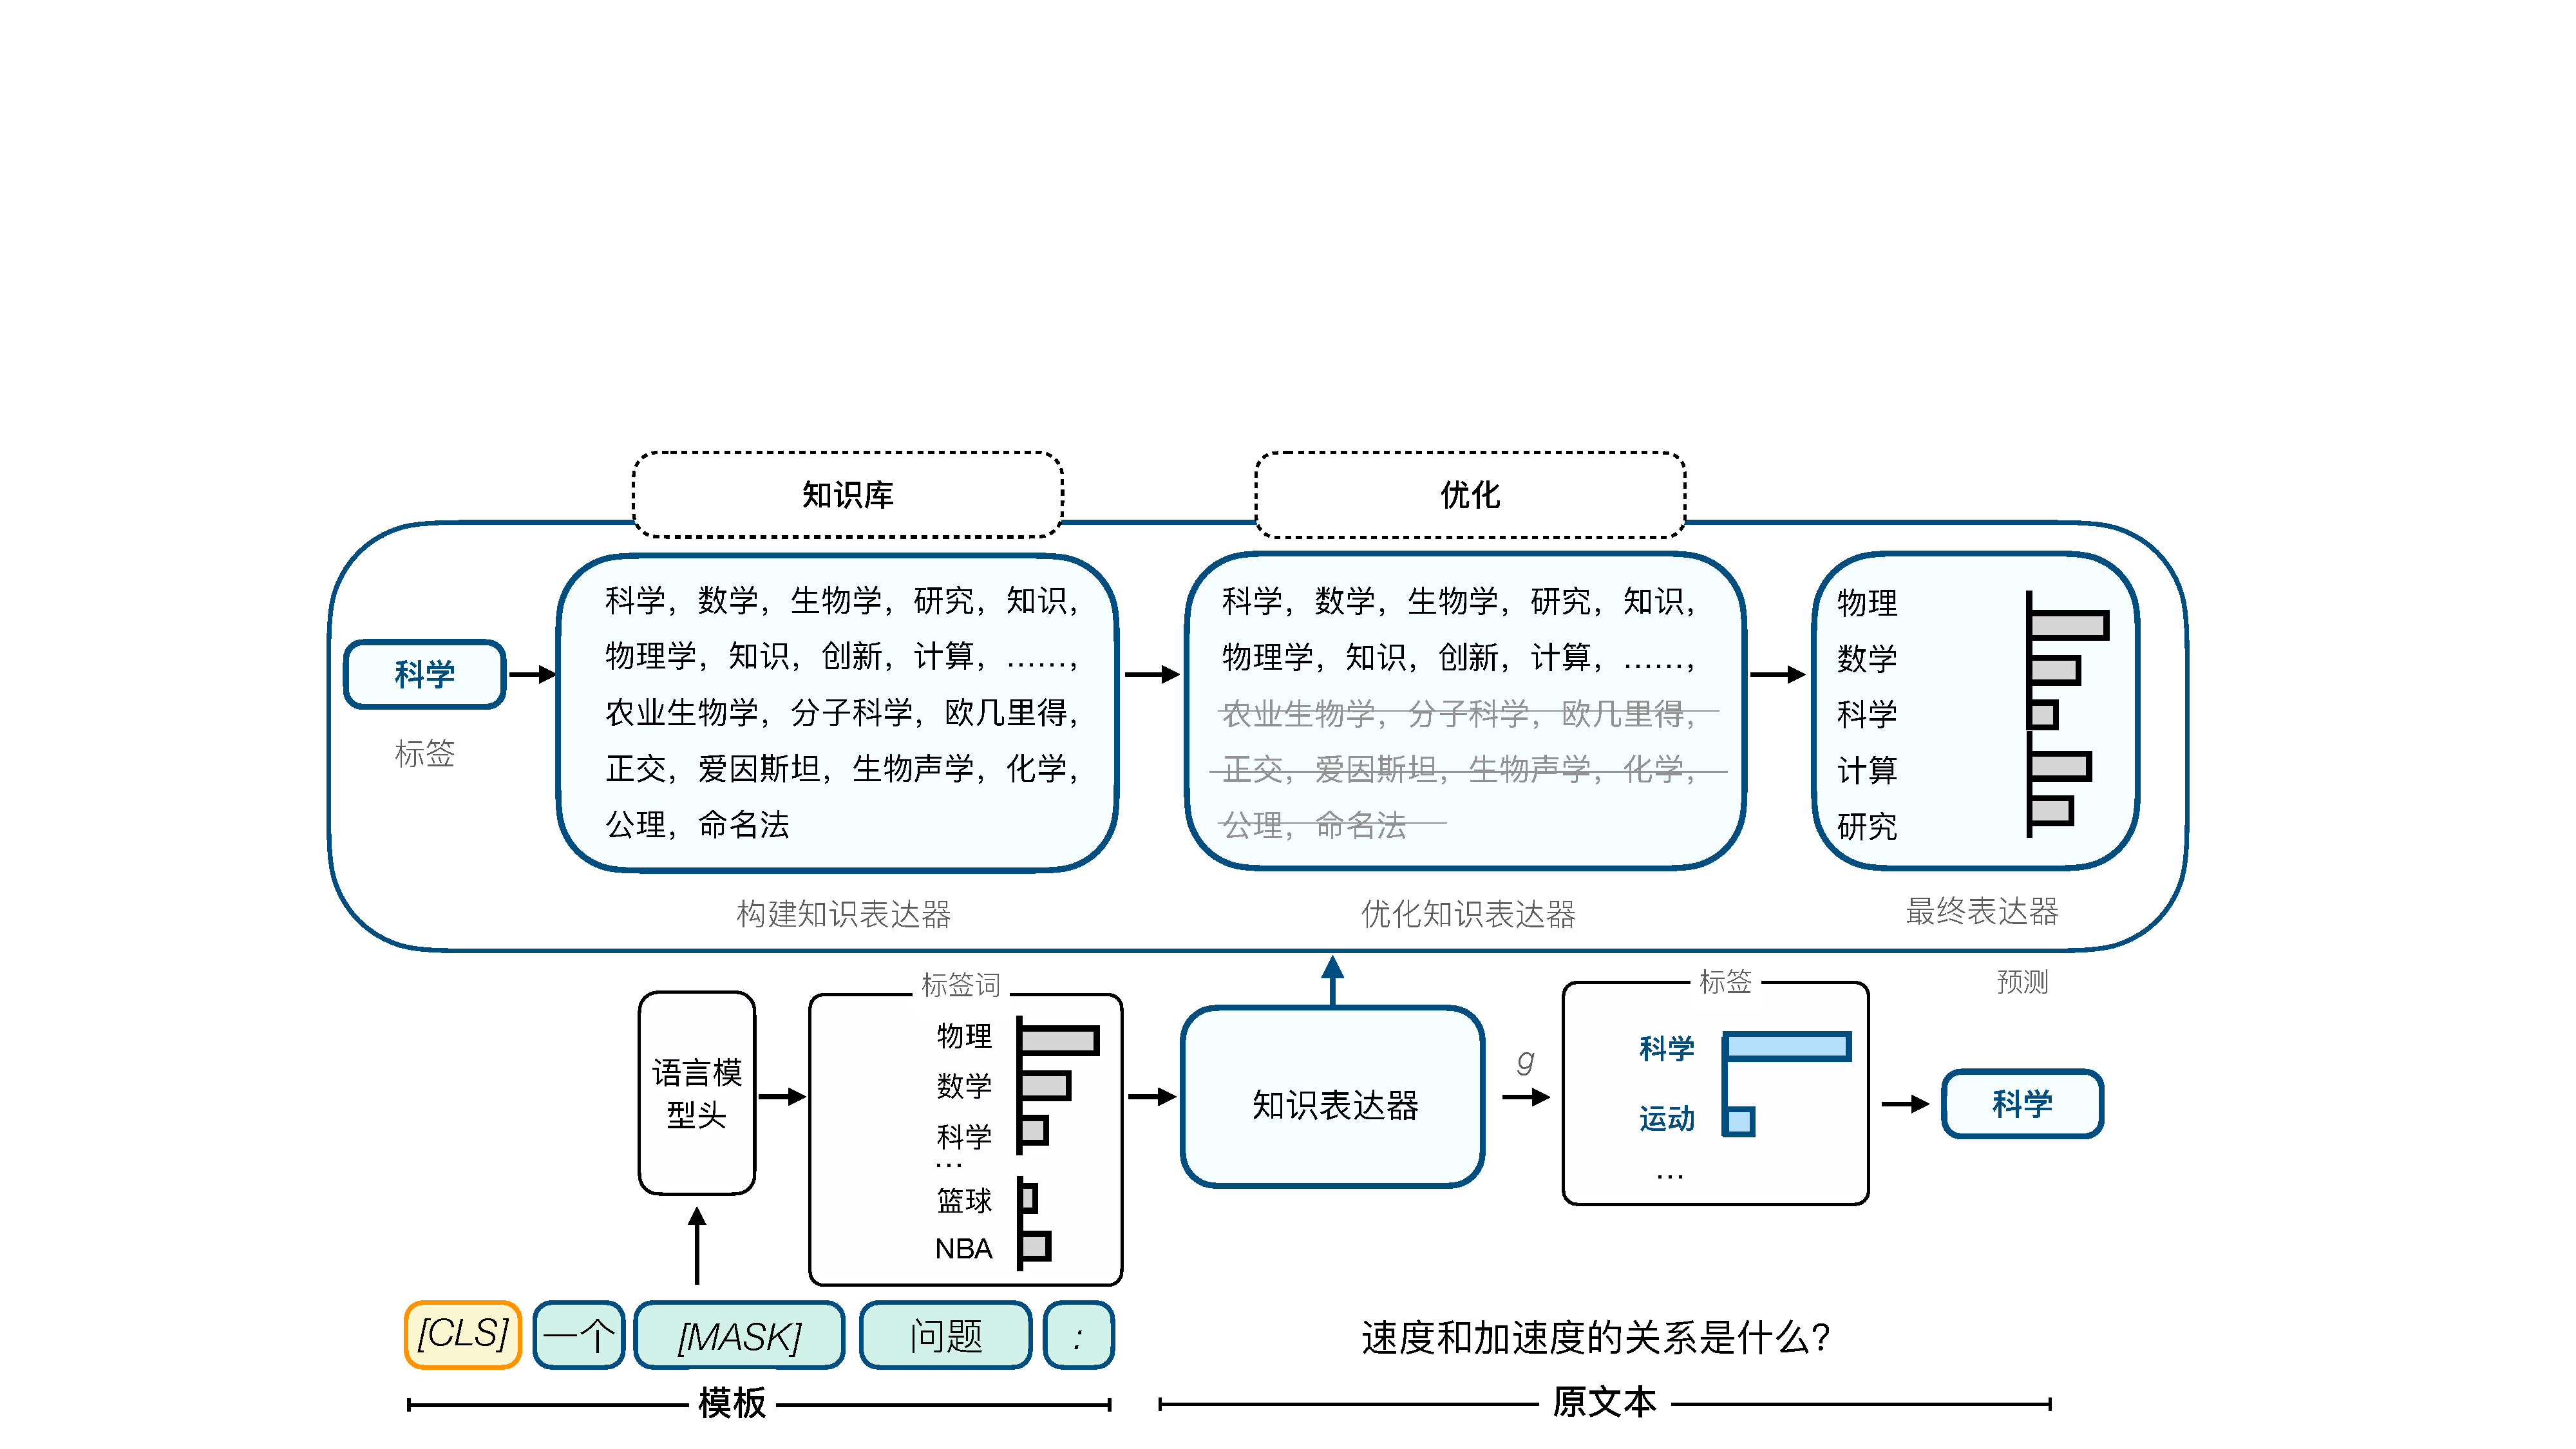
\includegraphics[width = \linewidth]{kptplots/framework_knowPrompt.pdf}
  }
  \caption{KPT框架示意图}
  \label{fig:my_label}
\end{figure*}


\subsubsection{语言表达器构建}
\label{sec:cons}

基于上下文预测掩码词的过程不是单一选择过程,即没有标准正确答案,而是有许多词可能适合该上下文。
因此,语言表达器映射的标签词应具备两个属性:\textit{广泛覆盖}和\textit{较少主观偏差}。这种全面的映射对于模仿预训练至关重要,而预训练是提示微调能力的来源。外部结构化知识可以同时满足这两个要求。在本节中,本文介绍了如何利用外部知识进行两种文本分类任务:主题分类和情感分类。

对于主题分类,核心问题是从所有方面和粒度中提取与主题相关的标签词。从这个角度出发,本文选择了Related Words~\footnote{\url{https://relatedwords.org}},这是一个从多个资源(包括词嵌入、ConceptNet~\cite{speer2017conceptnet}、WordNet~\cite{pedersen2004wordnet}等)聚合的知识图谱 $\mathcal{G}$ 作为外部知识库。
边表示“相关性”关系,并标注了相关性分数。本文假设每个类别的名称 $v_0$ 是正确的,并将其作为锚点获取邻域节点 $N_{\mathcal{G}}(v_0)$,其分数大于阈值 $\eta$ 作为相关词~\footnote{实验中取 $\eta=0$}。因此,每个类别被映射到一组标签词 $\mathcal{V}_{y} = N_{\mathcal{G}}(v_0) \cup \{v_0\}$。
对于二元情感分类,主要目标是扩展二元情感到更多粒度和方面的情感。本文使用了之前研究人员总结的情感词典~\footnote{\url{https://www.enchantedlearning.com/wordlist/positivewords.shtml}}$^{,}$\footnote{ \url{https://www.enchantedlearning.com/wordlist/negativewords.shtml}}。
KPT中标签词的几个示例如表~\ref{tab:label_words_examples}所示。

\begin{table*}[!htbp]
    \centering
    \caption{扩展标签词的示例。}
\scalebox{0.93}{
    \begin{tabular}{ccl}
    \toprule
  数据集 &  标签 & \multicolumn{1}{c}{标签词} \\
    \midrule
  \multirow{2}{*}{AG新闻数据集}  &  \textsc{政治} &  政治, 政府, 外交, 法律, 亚里士多德, 外交的, 治理 ...\\
    &  \textsc{体育}   & 体育, 运动, 体操, 运动员, 竞赛, 自行车, 足球 ... \\
      \midrule
 \multirow{2}{*}{IMDB数据集} &    \textsc{负面} & 糟糕的, 不利的, 令人担忧的, 生气的, 烦恼的, 焦虑的, 冷漠的, 可怕的 ...\\
    &  \textsc{正面} & 绝对的, 接受的, 备受赞誉的, 完成, 成就  ...\\
      \bottomrule
    \end{tabular}
}
    \label{tab:label_words_examples}
\end{table*}

\subsubsection{语言表达器优化}
\label{sec:refine}

尽管构建了一个包含全面标签词的知识化语言表达器,但由于知识库的词汇并非为预训练语言模型量身定制,收集的标签词可能非常嘈杂。因此,有必要通过保留高质量词来优化语言表达器。在本节中,本文提出了四种优化方法,分别解决嘈杂标签词的不同问题。

\textbf{频率优化。} 第一个问题是处理罕见词。本文假设知识库中的某些词对预训练语言模型来说是罕见的,因此这些词的预测概率往往不准确。我提出使用标签词的\emph{上下文先验}来去除这些词。具体来说,给定一个文本分类任务,本文表示语料库中句子 $\mathbf{x}$ 的分布为 $\mathcal{D}$。对于分布中的每个句子,我将其包裹到模板中,并计算每个标签词 $v$ 在掩码位置的预测概率 $P_{\mathcal{M}}(\texttt{[MASK]}\!\!\!=\!v|\mathbf{x}_{\text{p}})$。通过对整个句子分布的概率取期望,可以得到标签词在掩码位置的先验分布。将其形式化为

\begin{equation}
 P_{\mathcal{D}}(v)\! =\! \mathbb{E}_{\mathbf{x}\sim \mathcal{D}} P_{\mathcal{M}}(\texttt{[MASK]}\!\!\!=\!v|\mathbf{x}_{\text{p}}).
\end{equation}
根据经验,本文发现使用从训练集中采样的小规模\emph{未标注支持集} $\tilde{\mathcal{C}}$ 并去除标签,可以很好地估计上述期望。因此,假设输入样本 $\{\mathbf{x}\in \tilde{\mathcal{C}}\}$ 具有均匀先验分布,上下文先验近似为
\begin{equation}
    P_{\mathcal{D}}(v) \approx \frac{1}{|\tilde{\mathcal{C}}|} \sum_{\mathbf{x}\in \tilde{\mathcal{C}}} P_{\mathcal{M}}(\texttt{[MASK]}\!\!\!=\!v|\mathbf{x}_{\text{p}}),
\end{equation}
然后移除先验概率小于阈值的标签词。由于上下文化先验概率的绝对值分布可能因任务而异,确定一个具体的上下文化先验概率阈值可能会非常难以捉摸。本文采用基于排序的阈值,即过滤掉出现在上下文化先验概率下半部分的标签词。

\textbf{相关性优化。}
由于本文构建的知识化标签词是完全无监督的,某些标签词可能比其他词更相关于其所属类别。
为了衡量标签词与每个类别的相关性,本文获取标签词在支持集 $\tilde{\mathcal{C}}$ 上的预测概率作为标签词的向量表示 $\mathbf{q}^{v}$,即 $\mathbf{q}^{v}$ 的第 $i$ 个元素为

\begin{equation}
    \mathbf{q}^{v}_i = P_{\mathcal{M}}([\texttt{MASK}]=v|\mathbf{x}_{i{\text{p}}}), \mathbf{x}_i\in \tilde{\mathcal{C}},
\end{equation}
其中 $\mathbf{x}_{i{\text{p}}}$ 表示句子 $x_i$ 与模板 $\text{p}$ 的组合。

为了估计类别的表示,本文假设每个类别的名称 $v_0$(例如“科学”对于 \textsc{科学})虽然覆盖范围有限,但与类别非常相关。然后本文使用这些名称的向量表示 $\mathbf{q}^{v_0}$ 作为类别的表示 $\mathbf{q}^{y}$。因此,标签词 $v$ 与类别 $y$ 之间的相关性得分计算为两个表示之间的余弦相似度:
\begin{equation}
    r(v, y) = \operatorname{cos}(\mathbf{q}^{v}, \mathbf{q}^{y}) = \operatorname{cos}(\mathbf{q}^{v}, \mathbf{q}^{v_0}).
\end{equation}

此外,某些标签词可能对多个类别有积极贡献,导致类别之间的混淆。例如,类别 \textsc{科学} 的潜在标签词“生理学”也可能在类别 \textsc{体育} 的句子中被赋予高概率。为了减轻这种混淆并过滤相关性较低的标签词,本文设计了一个指标,该指标偏好仅对其所属类别具有高相关性且对其他类别相关性较低的标签词:
\begin{equation}
    R(v) = r(v, f(v)) \frac{|\mathcal{Y}|-1}{\sum_{y\in \mathcal{Y}, y\neq f(v)}(r(v,y))},
\label{equ: rr_tfidf}
\end{equation}
其中 $f(v)$ 是 $v$ 对应的类别。

理想情况下,一个好的标签词至少应具有对其所属类别的高于其他类别平均相关性得分的相关性得分。因此,本文移除 $R(v)<1$ 的标签词。在实践中,本文对公式~\eqref{equ: rr_tfidf} 进行了轻微修改,这是因为本文观察到在只有少数类别的分类任务中,提供一个更严格的标准以确保标签词对\emph{任何其他}类别的相关性得分低于其对所属类别的得分是更好的选择,即优先选择IDF得分中的\emph{最大值}。为了保持统一的标准,本文使用基于范数的IDF得分:
\begin{equation}
    R^d(v)\! =\! r(v, f(v)) \large(\frac{|\mathcal{Y}|-1}{\sum_{y\in \mathcal{Y}, y\neq f(v)} r(v,y)^d}\large)^{1/d},
\end{equation}
其中
\begin{equation}
    d = \frac{C}{|\mathcal{Y}|-2+\epsilon} +1, C>0.
\end{equation}
该标准会使用标签个数对相关性分布进行锐化,在只有少数标签的分类任务中会近似于$\{r(v,y)|y\in |\mathcal{Y}|, y\neq f(v)\}$中的最大值,而在处理多标签分类时会退化为公式~\eqref{equ: rr_tfidf}中的平均得分。实验中取$C=10$(未经试错调整),且$0 < \epsilon\ll 1$是一个防止数值错误的小数。


本质上,这种相关性优化采用了经典TF-IDF~\cite{jones1972statistical}算法的思想,该算法估计词与文档的相关性。它偏好使用对特定文档相关而对其他文档不相关的词作为文档的关键词。在KPT中,类别类似于文档,而标签词类似于文档中的词。从这个角度来看,公式~\eqref{equ: rr_tfidf} 是TF-IDF度量的一种变体。 


\textbf{上下文校准。}\quad
\label{sec: refine-CC}
第三个问题是标签词先验概率的显著差异。正如之前的工作~\cite{pmlr-v139-zhao21c, holtzman2021surface}所示,某些标签词无论输入句子的标签如何,被预测的概率都较低,导致预测偏差。在本文的设置中,知识库中的标签词往往具有更多样化的先验概率,导致问题更加严重(见表~\ref{tab:experiment-zero-shot})。因此,本文使用标签词的上下文先验来校准预测分布,即上下文校准(Contextual Calibration, 简称CC):
\begin{equation}
    \tilde{P}_{\mathcal{M}}(\!\texttt{[MASK]}\!\!\!=\!v|\mathbf{x}_{\text{p}}) \!\propto\! \frac{P_{\mathcal{M}}(\!\texttt{[MASK]}\!\!\!=\!v|\mathbf{x}_{\text{p}})}{P_{\mathcal{D}}(v)},
\end{equation}
其中 $P_{\mathcal{D}}(v)$ 是标签词的先验概率。最终概率归一化为1。

\textbf{可学习优化}。在少样本学习中,优化可以通过学习过程加强。具体来说,本文为每个标签词 $v$(可能已经通过上述方法优化)分配一个可学习权重 $w_v$。权重形成一个向量 $\mathbf{w}\in \mathbb{R}^{|\mathcal{V}|}$,初始化为零向量。权重在每个 $\mathcal{V}_y$ 内归一化:

\begin{equation}
    \alpha_v = \frac{\operatorname{exp}(w_v)}{\sum_{u\in \mathcal{V}_y} \operatorname{exp}(w_u)}.
\end{equation}

直观上,在训练过程中,预计会为嘈杂的标签词学习到一个较小的权重,以最小化其对预测的影响。需要注意的是,在少样本设置中,校准可能不是必需的,因为标签词的概率可以被训练到所需的幅度,即 $\tilde{P}_{\mathcal{M}}(\texttt{[MASK]}\!\!\!=\!v|\mathbf{x}_{\text{p}}) ={P_{\mathcal{M}}(\texttt{[MASK]}\!\!\!=\!v|\mathbf{x}_{\text{p}})}$。

除了这些优化方法外,由于许多标签词对预训练语言模型来说是词汇表外的,并且被分词器拆分为多个标记。对于这些词,本文简单地使用每个标记的平均预测得分作为词的预测得分。这种简单方法的影响在分析小节~\ref{app:experiment-st}中进行了研究。

\subsubsection{语言表达器利用}
\label{sec:use}

最后一个问题是如何将优化后的标签词的预测概率映射到类别标签 $y$。

\textbf{简单平均。} 优化后,本文可以假设每个类别的标签词对预测标签的贡献相等。因此,本文使用 $\mathcal{V}_y$ 上预测得分的平均值作为标签 $y$ 的预测得分。
预测标签 $\hat{y}$ 为

\begin{equation}
\hat{y}\!=\!
    \mathrm{arg}\!\max_{y\in\mathcal{Y}}\frac{\sum_{v \in \mathcal{V}_{y}}\! \tilde{P}_{\mathcal{M}}(\!\texttt{[MASK]}=v|\mathbf{x}_{\text{p}})}{|\mathcal{V}_y|}.
\end{equation}

本文在零样本学习中使用此方法,因为没有需要训练的参数。

\textbf{加权平均。} 在少样本设置中,借助可学习优化,本文采用标签词得分的加权平均作为预测得分。优化权重 $\alpha_v$ 用作平均的权重。因此,预测的 $\hat{y}$ 为
\begin{equation}
\hat{y} \!= \operatorname{argmax}_{y\in\mathcal{Y}} \frac{\exp\left({s(y|\mathbf{x}_{\text{p}})}\right)}{\sum_{y'}\exp\left({s({y'}|\mathbf{x}_{\text{p}})}\right)},
\end{equation}
其中 $s(y|\mathbf{x}_{\text{p}})$ 为
\begin{equation}
        s(y|\mathbf{x}_{\text{p}})\!=\!\! \sum_{v\in\mathcal{V}_y} \!\!\alpha_v  \operatorname{log}{P}_{\mathcal{M}}(\texttt{[MASK]}\!\!\!=\!v|\mathbf{x}_{\text{p}})。
\end{equation}

该目标函数适用于通过应用交叉熵损失对预测概率进行连续优化。


\subsubsection{KPT方法的理论分析}

在本节中,本文对KPT使用的整个框架进行了理论分析。在提示微调中,给定一个文本$\mathbf{x}$,将其包装到模板中以形成包装句子$\mathbf{x}_{\text{p}}$。然后使用预训练语言模型预测标签词$v$的概率:
\begin{equation}
% \small
    p(\texttt{[M]}\!\!\!=\!v|\mathbf{x}) = P_{\mathcal{M}}(\texttt{[M]}\!\!\!=\!v|\mathbf{x}_{\text{p}}),
\end{equation}
其中$\texttt{[M]}$是$\texttt{[MASK]}$的缩写,表示模板中掩码位置处标签词的预测。

如果使用多个标签词来表示单个标签,则通过边缘化所有标签词的预测概率来定义标签的预测概率,即:
\begin{align}
% \small
\begin{split}
  p(\text{Y}\!=\!y|\mathbf{x}) \!=\!\! \sum_{v\in V_{\mathcal{Y}}} p(\text{Y}\!=\!y, \texttt{[M]}\!\!\!=\!v|\mathbf{x}).
\end{split}
\label{appequ_1}
\end{align}

由于在给定$v$的情况下,Y的预测与$\mathbf{x}$无关,可以将公式~\eqref{appequ_1}改写为:
\begin{align}
\begin{split}
 &\sum_{v\in V_{\mathcal{Y}}} p(\text{Y}=y|\texttt{[M]}\!\!\!=\!v) p(\texttt{[M]}\!\!\!=\!v|\mathbf{x}) \\ 
 = & \sum_{v\in V_{\mathcal{Y}}}  p(\text{Y}=y|\texttt{[M]}\!\!\!=\!v) P_{\mathcal{M}}(\texttt{[M]}\!\!\!=\!v|\mathbf{x}_{\text{p}}).
 \end{split}
\label{appequ_21}
\end{align}

利用贝叶斯定理并假设分类问题是平衡的,公式~\eqref{appequ_21}可以转化为:
\begin{align}\label{appequ_2}
 &\sum_{v\in V_{\mathcal{Y}}} \frac{p(\texttt{[M]}\!\!\!=\!v|\text{Y}=y)p(\text{Y}=y) }{p(\texttt{[M]}\!\!\!=\!v)} P_{\mathcal{M}}(\texttt{[M]}\!\!\!=\!v|\mathbf{x}_{\text{p}})\nonumber\\
 &\propto \!\! \sum_{v\in V_{\mathcal{Y}}}\! \frac{p(\texttt{[M]}\!\!\!=\!v|\text{Y}=y)}{p(\texttt{[M]}\!\!\!=\!v)} P_{\mathcal{M}}(\texttt{[M]}\!\!\!=\!v|\mathbf{x}_{\text{p}}). 
\end{align}

现在,标签的预测概率由三部分组成。

(1) 第一部分$p(v|\text{Y}=y)$是在给定类别标签$y$的情况下预测特定标签词$v$的概率。直观上,如果标签词与标签$y$相关,则该概率值会较高。在KPT中,\textbf{相关性优化}通过量化目标估计该概率,即如果相关性得分超过阈值$1$,则保留该值,否则将其过滤。另一方面,\textbf{可学习优化}通过连续权重估计该概率。

(2) 第二部分是分母中的$p(\texttt{[M]}\!\!\!=\!v)$。该术语实际上是标签词$v$的先验概率,由\textbf{上下文校准}估计。之前的工作也尝试通过上下文无关的方式处理该术语~\cite{holtzman2021surface, pmlr-v139-zhao21c}。

(3) 最后一项$P_{\mathcal{M}}(\texttt{[MASK]}\!\!\!=\!v|\mathbf{x}_{\text{p}})$是由PLM预测的标签词$v$的概率,这是大多数工作中唯一的组成部分,例如手动语言表达器~\cite{schick2020exploiting},与KPT相比,这些方法得到的解决方案是次优的。

因此,只要使用公式~\eqref{appequ_1}作为其核心假设,所有使用多个标签词表示类别标签的语言表达器都可以形式化到该框架中。然而,据本文所知,KPT是第一个将这三个组成部分结合起来形成强大语言表达器的方法。



\subsection{实验}
本文在五个文本分类数据集上评估了KPT,以展示将外部知识融入提示微调的有效性。

\subsubsection{数据集与模板}

实验在三个主题分类数据集上进行:AG新闻数据集~\cite{zhang2015character}、DBPedia数据集~\cite{lehmann2015dbpedia}和雅虎数据集~\cite{zhang2015character},以及两个情感分类数据集:IMDB数据集~\cite{maas2011learning}和亚马逊数据集~\cite{mcauley2013hidden}。数据集的统计信息如表~\ref{tab:dataset_stat}所示。每个数据集的详细信息和统计数据见表\ref{tab:dataset_stat}。

\begin{table}[!htbp]
    \centering
    \caption{KPT使用的各数据集的统计信息}
    \scalebox{1}{
    \begin{tabular}{cccc}
\toprule
    名称 & 类型 & 类别数 & 测试集大小 \\ 
\midrule
      AG新闻数据集   & 主题  & 4 & 7600 \\
       DBPedia数据集  & 主题  & 14 & 70000 \\
       雅虎数据集 & 主题 & 10 & 60000 \\
       亚马逊数据集 & 情感  & 2 & 10000 \\
       IMDB数据集 & 情感  & 2 & 25000 \\
     \bottomrule
    \end{tabular}
    }
    \label{tab:dataset_stat}
\end{table}

由于手动模板包含丰富的专家知识,尽管构建简单,但其表现已被证明优于或至少不逊色于自动生成的模板~\cite{gao2020making}。因此,本文在实验中使用手动模板。在零样本设置中,手动模板也比自动生成的模板更具适用性。为了减少不同模板的影响,本文在每种实验配置下测试了KPT在四种手动模板下的表现,这些模板要么由~\cite{schick2020exploiting}引入,要么根据数据集进行了调整。各数据集的介绍以及对应的模板如下。

\textbf{AG新闻数据集}。AG新闻数据集 是一个新闻主题分类数据集。本文遵循 PET~\cite{schick2020exploiting} 设计模板。然而,其最佳性能的模板 $T$(\textbf{x}) =  ``\texttt{[MASK]} news : \textbf{x}'' 要求 \texttt{[MASK]} 标记大写,这不适用于知识库中的标签词。此外,部分模板信息量不足,表现较差。因此,本文定义了四个稍作修改的模板:

\newtcolorbox{mybox}{colback=gray!6!white, colframe=gray!75!black, width=0.75\textwidth}
\newtcolorbox{mybox2}{colback=gray!6!white, colframe=gray!75!black, width=0.75\textwidth}
\newtcolorbox{mybox3}{colback=gray!6!white, colframe=gray!75!black, width=0.75\textwidth}


{\centering
\begin{mybox}
\begin{align*}
 T_1(\mathbf{x}) &= \text{ A \texttt{[MASK]} news:} \mathbf{x} \\
 T_2(\mathbf{x}) &= \mathbf{x} \text{ This topic is about \texttt{[MASK]} .}\\
  T_3(\mathbf{x}) &=  \text{ [ Category :\texttt{[MASK]} ]} \mathbf{x}\\
  T_4(\mathbf{x}) &=  \text{ [ Topic :\texttt{[MASK]} ]} \mathbf{x}
\end{align*}
\end{mybox}
}

\textbf{DBPedia数据集}。在 DBPedia数据集 样本中,给定一个段落 $\mathbf{b}$ 和标题 $\mathbf{a}$,其中标题是段落的主题。任务是确定主题的类型。与其他主题分类不同,段落可能强调与标题不同的主题。例如,在一段关于音频公司的段落中,主要内容涉及音乐、专辑等,但正确的标签是“公司”而非“音乐”。因此,本文定义了以下模板:

{\centering
\begin{mybox2}
\begin{align*}
     T_1(\mathbf{a},\mathbf{b}) &=  \mathbf{a} \ \mathbf{b}  \  \tilde{\mathbf{a}}  \text{ is a \texttt{[MASK]} . }\\
      T_2(\mathbf{a},\mathbf{b}) &=  \mathbf{a} \   \mathbf{b}  \  \text{ In this sentence, } \  \tilde{\mathbf{a}}  \text{ is a \texttt{[MASK]} . } \\
   T_3(\mathbf{a},\mathbf{b}) &=   \mathbf{a}\ \mathbf{b} \  \text{The type of}\  \tilde{\mathbf{a}} \ \text{is}\  \texttt{[MASK]} .\\
   T_4(\mathbf{a},\mathbf{b}) &=\mathbf{a}\ \mathbf{b} \ \text{The category of}\  \tilde{\mathbf{a}} \ \text{is}\ \texttt{[MASK]} .
\end{align*}
\end{mybox2}
}
其中 $\tilde{\mathbf{a}}$ 表示去除标题中的最后一个标点符号。

\textbf{雅虎数据集}。 雅虎数据集是一个关于雅虎网站提问的主题分类数据集~\cite{zhang2015character}。本文使用与 AG新闻数据集 相同的模板,只是将 $T_1(\mathbf{x})$ 中的“news”改为“question”:

{\centering
\begin{mybox}
\begin{align*}
     T_1(\mathbf{x})  &= \text{ A \texttt{[MASK]} question : }  \mathbf{x}  \\
     T_2(\mathbf{x})  &= \mathbf{x} \text{ This topic is about \texttt{[MASK]}. }\\
     T_3(\mathbf{x})   &= \text{ [ Category : \texttt{[MASK]} ] }  \mathbf{x}  \\
     T_4(\mathbf{x})   &=\text{ [ Topic : \texttt{[MASK]} ] } \mathbf{x} 
\end{align*}
\end{mybox}
}

\textbf{IMDB数据集}。 IMDB数据集 是一个关于电影评论的情感分类数据集。类似于~\cite{schick2020exploiting}中为情感分类定义的模板,本文定义了以下模板:

{\centering
\begin{mybox3}
\begin{align*}
       T_1(\mathbf{x}) & = \text{ It was \texttt{[MASK]} . } \mathbf{x}\\
    T_2(\mathbf{x}) &  = \text{ Just \texttt{[MASK]} ! } \mathbf{x}\\
      T_3(\mathbf{x}) & = \mathbf{x} \text{ All in all, it was } \texttt{[MASK]} . \\
      T_4(\mathbf{x}) & = \mathbf{x} \text{ In summary, the film was } \texttt{[MASK]}.  
\end{align*}
\end{mybox3}
}

\textbf{亚马逊数据集}。 亚马逊数据集 是另一个情感分类数据集,本文定义了以下模板:

{\centering
\begin{mybox}
\begin{align*}
       T_1(\mathbf{x}) & = \text{ It was \texttt{[MASK]} } .\  \mathbf{x}\\
    T_2(\mathbf{x}) &  = \text{ Just \texttt{[MASK]} ! } \mathbf{x}\\
      T_3(\mathbf{x}) & = \mathbf{x} \text{ All in all, it was  \texttt{[MASK]}} . \\
      T_4(\mathbf{x}) & = \mathbf{x} \text{ In summary, it was  \texttt{[MASK]}} ".  
\end{align*}
\end{mybox}
}

由于 亚马逊数据集 的测试集过大,本文从 400,000 个测试样本中随机抽取 10,000 个样本进行测试,预实验表明这对性能影响极小。



\subsubsection{实验设置}
实验基于OpenPrompt~\cite{ding2021openprompt}进行,这是一个我参与开发的提示学习开源工具包。预训练语言模型使用$\text{RoBERTa}_\text{large}$~\cite{liu2019roberta}。测试指标在所有实验中使用Micro-F1。对于所有零样本实验,如果实验中引入了随机性,则使用不同的随机种子重复实验3次;对于所有少样本实验,重复5次。需要注意的是,考虑到四种模板和五/三个随机种子,每个基于提示的方法的得分是20/12次实验的平均值,这大大降低了评估结果的随机性。基于支持集$\tilde{\mathcal{C}}$的优化中,未标注支持集的大小$|\tilde{\mathcal{C}}|$为200。对于少样本学习,实验设置了1、5、10和20样本。在$k$样本实验中,从原始训练集中为每个类别采样$k$个实例组成少样本训练集,并采样另外$k$个实例组成验证集。整个模型训练5个epoch,并选择验证性能最佳的检查点进行测试。其他超参数见表~\ref{tab:app_exp_settings}。对于软提示词,本文使用 $3e-4$ 的学习率来加速其软标签词嵌入的收敛。

\begin{table}[!htbp]
    \centering
    \begin{tabular}{p{0.3\textwidth}p{0.4\textwidth}p{0.1\textwidth}}
\toprule
      超参数  & 数据集 & 值 \\
\midrule
   截断长度  & AG新闻数据集, DBPedia数据集, 雅虎数据集    &  128 \\
截断长度  & 亚马逊数据集, Imdb    &  512 \\
   预热步数 & 全部 & 0 \\
   学习率 & 全部 & 3e-5 \\
   最大训练轮数 & 全部 & 5\\
   Adam epsilon & 全部 & 1e-8 \\
\bottomrule
    \end{tabular}
    \caption{超参数设置}
    \label{tab:app_exp_settings}
\end{table}




\subsubsection{基线方法}
在本小节中,本文介绍了用于对比的基线方法。为了更好地理解本文提出的方法,本文还比较了KPT在不同配置下的性能,也在下面列为基线。

\textbf{微调(FT)。}\quad 传统的微调方法将预训练语言模型的\texttt{[CLS]}标记的隐藏嵌入输入分类层以进行预测。需要注意的是,微调方法不能应用于零样本设置,因为分类层是随机初始化的。

\textbf{提示微调(PT)。}\quad 常规的提示微调方法使用类名作为每个类的唯一标签词,这种方法在PET~\cite{schick2020exploiting}和大多数现有工作中使用。为了公平比较,本文未使用PET中的技巧,例如自训练和提示集成,因为这些技巧与本文的贡献正交。

\textbf{自动标签词生成器(AUTO)。}\quad 自动标签词生成器由PETAL~\cite{schick2020automatically}提出,它使用有标注数据从预训练语言模型的词汇表中选择信息量最大的标签词。该方法适用于没有手动定义类名的情况。目前尚不清楚如何将其与手动定义的类名结合以提升性能,以及如何在零样本设置中应用。因此,本文仅在少样本设置中且未提供类名信息的情况下进行比较。

\textbf{软标签词生成器(SOFT)。}\quad 软标签词生成器由WARP~\cite{hambardzumyan-etal-2021-warp}提出。他们为每个类使用一个连续向量,并通过掩码语言模型输出与类向量的点积来生成每个类的概率。在实验中,其类向量使用类名的词嵌入初始化,因为使用手动类名作为初始值更有效(见\ref{app:soft-pilot}小节的预实验)。作为一种基于优化的方法,软标签词生成器不适用于零样本设置。

\textbf{PT+CC。} 对于零样本设置,本文进一步引入了结合上下文校准的PT作为基线,以观察上下文校准相较于知识化标签词生成器的改进程度\footnote{使用的支持集与KPT相同。}。

对于\textbf{KPT},本文实验了不同变体以更好地理解所提出的方法,例如优化。\textbf{-FR}、\textbf{-RR}、\textbf{-CC}和\textbf{-LR}分别表示不进行频率优化、相关性优化、上下文校准和可学习优化的变体。在少样本实验中,本文假设监督训练数据可以将每个标签词的输出概率训练到所需的幅度,因此在KPT中未使用CC和FR。这一决定的合理性在小节\ref{app:fewshot-cali}中进行了说明。


\subsubsection{预实验}
% \onecolumngrid
\begin{table}[!htbp]
\caption{预实验证明了在语言表达器中融入人类专家知识的必要性}
\begin{center}
\scalebox{0.72}{
\begin{tabular}{lllllll}
\toprule
示例数 & 方法  & AG新闻数据集   & DBPedia数据集 & 雅虎数据集 & 亚马逊数据集 & IMDB数据集  \\
\midrule
\multirow{2}{*}{5} & SOFT &82.8 $\pm$ 2.7 \smallcolor{(84.3)} & 97.0 $\pm$ 0.6 \smallcolor{(97.2)} & 61.8 $\pm$ 1.8 \smallcolor{(63.1)} & 93.2 $\pm$ 1.6 \smallcolor{({94.2})} & 91.6 $\pm$ 3.4 \smallcolor{({93.9})} \\
& SOFT w.o. M & 63.4 $\pm$ 11.3 \smallcolor{(64.7)} & 82.1 $\pm$ 5.9 \smallcolor{(86.1)} & 24.5 $\pm$ 6.2 \smallcolor{(27.2)} & 79.2 $\pm$ 10.5 \smallcolor{(85.5)} & 83.6 $\pm$ 11.5 \smallcolor{(93.4)} \\
\midrule
\multirow{2}{*}{10} & SOFT &85.0 $\pm$ 2.8 \smallcolor{(86.7)} & 97.6 $\pm$ 0.4 \smallcolor{(97.8)} & 64.5 $\pm$ 2.2 \smallcolor{(65.0)} & 93.9 $\pm$ 1.7 \smallcolor{(93.9)} & 91.8 $\pm$ 2.6 \smallcolor{(93.0)} \\
& SOFT w.o. M & 77.4 $\pm$ 4.8 \smallcolor{(79.1)} & 94.9 $\pm$ 2.5 \smallcolor{(95.9)} & 42.6 $\pm$ 8.3 \smallcolor{(48.1)} & 92.9 $\pm$ 2.0 \smallcolor{(94.0)} & 88.7 $\pm$ 9.7 \smallcolor{(93.8)} \\
\bottomrule
\end{tabular}}
\end{center}
\label{app:soft-pilot}
\end{table}

根据~\citep{gao2020making}指出的,手动定义的语言表达器比自动搜索/优化的语言表达器更具竞争力,甚至表现更好,这进一步加强了本文通过注入更多外部人类知识来改进手动语言表达器的动机。为了进一步说明手动语言表达器的优势,本文在soft 语言表达器中进行了初步实验。软语言表达器~\cite{hambardzumyan-etal-2021-warp}可以使用预定义的类别名称作为标签词进行初始化,本文将其作为基线方法列在表~\ref{tab:experiment-few-shot}中。它也可以在没有手动定义类别名称的情况下随机初始化。本文在5-shot和10-shot实验中测试了带有和不带有手动定义类别名称的Soft 语言表达器的性能。表~\ref{app:soft-pilot}中展示了这一结果。SOFT是使用类名的软语言表达器,而SOFT w.o. M是不使用手动语言表达器的变体。可以看出,两者之间的差距通常较大。因此,进一步改进带有手动定义类别名称的语言表达器比没有任何人类先验的从零学习的语言表达器更具前景。



\begin{table*}[!htbp]
  \caption{零样本文本分类的结果}
  \begin{center}
  \scalebox{0.82}{
  \begin{tabular}{lccccc}
  \toprule
   方法 & AG新闻数据集   & DBPedia数据集 & 雅虎数据集& 亚马逊数据集 & IMDB数据集  \\
  \midrule
  PT & 75.1 $\pm$ 6.2 \smallcolor{(79.0)} & 66.6 $\pm$ 2.3 \smallcolor{(68.4)} & 45.4 $\pm$ 7.0 \smallcolor{(52.0)} & 80.2 $\pm$ 8.8 \smallcolor{(87.8)} & 86.4 $\pm$ 4.0 \smallcolor{(92.0)} \\
  PT+CC & 79.9 $\pm$ 0.7 \smallcolor{(81.0)} & 73.9 $\pm$ 4.9 \smallcolor{(82.6)} & 58.0 $\pm$ 1.4 \smallcolor{(58.8)} & 91.4 $\pm$ 1.6 \smallcolor{(93.5)} & 91.6 $\pm$ 3.0 \smallcolor{(93.7)} \\
  \midrule
  KPT & \textbf{84.8 $\pm$ 1.2} \smallcolor{\smallcolor{(\textbf{86.7})}} & \textbf{82.2 $\pm$ 5.4} \smallcolor{(\textbf{87.4})} & \textbf{61.6 $\pm$ 2.2} \smallcolor{(\textbf{63.8})} & \textbf{92.8 $\pm$ 1.2} \smallcolor{(\textbf{94.6})} & \textbf{91.6 $\pm$ 2.7} \smallcolor{(94.0)} \\
   \cdashline{2-6}
  \ \ -FR & 82.7 $\pm$ 1.5 \smallcolor{(85.0)} & 81.8 $\pm$ 4.6 \smallcolor{(86.2)} & 60.9 $\pm$ 1.5 \smallcolor{(62.7)} & \textbf{92.8 $\pm$ 1.2} \smallcolor{(\textbf{94.6})} & 91.6 $\pm$ 2.8 \smallcolor{(\textbf{94.1})} \\
  \ \ \ \ -RR & 81.4 $\pm$ 1.5 \smallcolor{(83.7)} & 81.4 $\pm$ 4.5 \smallcolor{(85.8)} & 60.1 $\pm$ 1.0 \smallcolor{(61.4)} & \textbf{92.8 $\pm$ 1.2} \smallcolor{(\textbf{94.6})} & 91.6 $\pm$ 2.8 \smallcolor{(\textbf{94.1})} \\
  \ \ \ \ \ \ -CC & 55.5 $\pm$ 2.8 \smallcolor{(58.3)} & 64.5 $\pm$ 6.8 \smallcolor{(73.0)} & 42.4 $\pm$ 5.0 \smallcolor{(46.8)} &
  86.2 $\pm$ 5.7 \smallcolor{(92.5)} & 90.3 $\pm$ 2.8 \smallcolor{(\textbf{94.1})} \\
  \bottomrule
  \end{tabular}}
  \end{center}
  \label{tab:experiment-zero-shot}
  \end{table*}
  

\begin{table*}[!ht]
  \caption{1/5/10/20 样本文本分类的结果如下
  }
  \begin{center}
  \scalebox{0.72}{
  \begin{tabular}{lllllll}
  \toprule
  样本数 & 方法  & AG新闻数据集   & DBPedia数据集 & 雅虎数据集 & 亚马逊数据集 & IMDB数据集  \\
  \midrule
  \multirow{8}{*}{1} & FT & 19.8 $\pm$ 10.4 & 8.6 $\pm$ 4.5 &11.1 $\pm$ 4.0 & 49.9 $\pm$ 0.2 & 50.0 $\pm$ 0.0  \\
   & PT & 80.0 $\pm$ 6.0 \smallcolor{\smallcolor{(84.4)}} & 92.2 $\pm$ 2.5 \smallcolor{\smallcolor{(94.3)}} & 54.2 $\pm$ 3.1 \smallcolor{\smallcolor{(55.7)}} & 91.9 $\pm$ 2.7 \smallcolor{\smallcolor{(93.2)}} & 91.2 $\pm$ 3.7 \smallcolor{\smallcolor{(93.7)}} \\
  & AUTO & 52.8 $\pm$ 9.8 \smallcolor{\smallcolor{(57.6)}} & 63.0 $\pm$ 8.9 \smallcolor{\smallcolor{(68.3)}} & 23.3 $\pm$ 4.5 \smallcolor{\smallcolor{(25.0)}} & 66.6 $\pm$ 12.5 \smallcolor{\smallcolor{(72.7)}} & 75.5 $\pm$ 15.5 \smallcolor{\smallcolor{(83.1)}} \\
  & SOFT & 80.0 $\pm$ 5.6 \smallcolor{\smallcolor{(82.4)}} & 92.3 $\pm$ 2.3 \smallcolor{\smallcolor{(93.3)}} & 54.3 $\pm$ 2.7 \smallcolor{\smallcolor{(55.9)}} & 90.9 $\pm$ 5.8 \smallcolor{\smallcolor{(93.6)}} & 89.4 $\pm$ 8.9 \smallcolor{\smallcolor{(93.1)}} \\
   \cmidrule{2-7}
  & KPT & \textbf{83.7 $\pm$ 3.5} \smallcolor{\smallcolor{(\textbf{84.6})}} & \textbf{93.7 $\pm$ 1.8} \smallcolor{\smallcolor{(\textbf{95.3})}} & \textbf{63.2 $\pm$ 2.5} \smallcolor{\smallcolor{(\textbf{64.1})}} & 93.2 $\pm$ 1.3 \smallcolor{\smallcolor{(\textbf{93.9})}} & 92.2 $\pm$ 3.0 \smallcolor{\smallcolor{(\textbf{93.6})}} \\
  \cdashline{2-7}
  & \ \ - LR & 83.5 $\pm$ 3.8 \smallcolor{\smallcolor{(84.3)}} & 93.0 $\pm$ 1.8 \smallcolor{\smallcolor{(94.5)}} & 62.2 $\pm$ 2.9 \smallcolor{\smallcolor{(63.6)}} & \textbf{93.3 $\pm$ 1.3} \smallcolor{\smallcolor{(\textbf{93.9})}} & 92.2 $\pm$ 2.8 \smallcolor{\smallcolor{(\textbf{93.6})}} \\
  & \ \ - RR & 82.2 $\pm$ 3.2 \smallcolor{\smallcolor{(82.6)}} & 92.9 $\pm$ 1.8 \smallcolor{\smallcolor{(94.1)}} & 61.3 $\pm$ 4.2 \smallcolor{\smallcolor{(62.5)}} & 93.1 $\pm$ 1.5 \smallcolor{\smallcolor{(93.7)}} & \textbf{92.6 $\pm$ 1.7} \smallcolor{\smallcolor{(\textbf{93.6})}} \\
  & \ \ - RR - LR & 81.8 $\pm$ 3.3 \smallcolor{\smallcolor{(82.5)}} & 91.3 $\pm$ 1.7 \smallcolor{\smallcolor{(92.6)}} & 60.7 $\pm$ 4.2 \smallcolor{\smallcolor{(61.4)}} & 93.2 $\pm$ 1.5 \smallcolor{\smallcolor{(93.9)}} & 92.6 $\pm$ 1.5 \smallcolor{\smallcolor{(93.5)}} \\
  \midrule
  \multirow{8}{*}{5} & FT &  37.9 $\pm$ 10.0  & 95.8 $\pm$ 1.3  & 25.3 $\pm$ 14.2 & 52.1 $\pm$ 1.3     &  51.4 $\pm$ 1.4 \\
   & PT & 82.7 $\pm$ 2.7 \smallcolor{\smallcolor{(84.0)}} & 97.0 $\pm$ 0.6 \smallcolor{\smallcolor{(\textbf{97.3})}} & 62.4 $\pm$ 1.7 \smallcolor{\smallcolor{(63.9)}}  & 92.2 $\pm$ 3.3 \smallcolor{\smallcolor{(93.5)}} & 91.9 $\pm$ 3.1 \smallcolor{\smallcolor{(92.7)}} \\
  & AUTO &72.2 $\pm$ 10.1 \smallcolor{\smallcolor{(75.6)}} & 88.8 $\pm$ 3.9 \smallcolor{\smallcolor{(91.5)}} & 49.6 $\pm$ 4.3 \smallcolor{(51.2)} & 87.5 $\pm$ 7.4 \smallcolor{(90.8)} & 86.8 $\pm$ 10.1 \smallcolor{(92.1)} \\
  & SOFT &82.8 $\pm$ 2.7 \smallcolor{(84.3)} & 97.0 $\pm$ 0.6 \smallcolor{(97.2)} & 61.8 $\pm$ 1.8 \smallcolor{(63.1)} & 93.2 $\pm$ 1.6 \smallcolor{(\textbf{94.2})} & 91.6 $\pm$ 3.4 \smallcolor{(\textbf{93.9})} \\
   \cmidrule{2-7}
  & KPT & 85.0 $\pm$ 1.2 \smallcolor{(\textbf{85.9})} & 97.1 $\pm$ 0.4 \smallcolor{(97.3)} & \textbf{67.2 $\pm$ 0.8} \smallcolor{(\textbf{67.8})} & 93.4 $\pm$ 1.9 \smallcolor{(94.1)} & 92.7 $\pm$ 1.5 \smallcolor{(92.9)} \\
  \cdashline{2-7}
  &\ \ - LR & \textbf{85.1 $\pm$ 1.0} \smallcolor{(85.8)} & 97.1 $\pm$ 0.4 \smallcolor{(97.2)} & 67.0 $\pm$ 1.1 \smallcolor{(67.5)} & 93.4 $\pm$ 1.9 \smallcolor{(94.1)} & 92.8 $\pm$ 1.5 \smallcolor{(93.0)} \\
  &\ \ - RR & 84.3 $\pm$ 1.8 \smallcolor{(84.9)} & \textbf{97.2 $\pm$ 0.4} \smallcolor{(\textbf{97.3})} & \textbf{67.2 $\pm$ 0.8} \smallcolor{(67.7)} & \textbf{93.6 $\pm$ 1.4} \smallcolor{(94.1)} & \textbf{93.0 $\pm$ 2.0} \smallcolor{(93.8)} \\
  & \ \ - RR - LR & 84.2 $\pm$ 1.7 \smallcolor{(84.5)} & 97.1 $\pm$ 0.4 \smallcolor{(97.3)} & 66.6 $\pm$ 1.4 \smallcolor{(67.5)} & 93.4 $\pm$ 2.0 \smallcolor{(94.1)} & 93.0 $\pm$ 2.1 \smallcolor{(93.8)} \\
  \midrule
  \multirow{8}{*}{10} & FT & 75.9 $\pm$ 8.4   & 93.8 $\pm$ 2.2 & 43.8 $\pm$ 17.9 & 83.0 $\pm$ 7.0    & 76.2 $\pm$ 8.7  \\
   & PT & 84.9 $\pm$ 2.4 \smallcolor{(86.1)} & 97.6 $\pm$ 0.4 \smallcolor{(97.8)} & 64.3 $\pm$ 2.2 \smallcolor{(64.8)} & 93.9 $\pm$ 1.3 \smallcolor{(94.6)} & \textbf{93.0 $\pm$ 1.7} \smallcolor{(\textbf{94.0})} \\
   & AUTO & 81.4 $\pm$ 3.8 \smallcolor{(84.1)} & 91.5 $\pm$ 3.4 \smallcolor{(95.1)} & 58.7 $\pm$ 3.1 \smallcolor{(60.9)} & 93.7 $\pm$ 1.2 \smallcolor{(94.5)} & 91.1 $\pm$ 5.1 \smallcolor{(93.3)} \\
   & SOFT &85.0 $\pm$ 2.8 \smallcolor{(86.7)} & 97.6 $\pm$ 0.4 \smallcolor{(97.8)} & 64.5 $\pm$ 2.2 \smallcolor{(65.0)} & 93.9 $\pm$ 1.7 \smallcolor{(93.9)} & 91.8 $\pm$ 2.6 \smallcolor{(93.0)} \\
  %  \cmidrule{2-6}
   \cmidrule{2-7}
  & KPT & \textbf{86.3 $\pm$ 1.6} \smallcolor{(87.0)} & \textbf{98.0 $\pm$ 0.2} \smallcolor{(\textbf{98.1})} & \textbf{68.0 $\pm$ 0.6} \smallcolor{(\textbf{68.2})} & 93.8 $\pm$ 1.2 \smallcolor{(94.1)} & 92.9 $\pm$ 1.8 \smallcolor{(93.3)} \\
  \cdashline{2-7}
  & \ \ - LR & 85.9 $\pm$ 1.9 \smallcolor{(\textbf{87.1})} & 98.0 $\pm$ 0.2 \smallcolor{(\textbf{98.1})} & 67.9 $\pm$ 0.7 \smallcolor{(\textbf{68.2})} & 93.9 $\pm$ 1.1 \smallcolor{(94.1)} & \textbf{93.0 $\pm$ 1.7} \smallcolor{(93.2)} \\
  & \ \ - RR & 85.6 $\pm$ 1.4 \smallcolor{(86.2)} & 97.9 $\pm$ 0.2 \smallcolor{(98.0)} & 67.5 $\pm$ 1.1 \smallcolor{(68.1)} & {94.0 $\pm$ 1.0} \smallcolor{(\textbf{94.7})} & 92.7 $\pm$ 2.1 \smallcolor{(93.0)} \\
  & \ \ - RR - LR & 85.1 $\pm$ 1.4 \smallcolor{(86.0)} & 97.8 $\pm$ 0.2 \smallcolor{(97.8)} & 66.8 $\pm$ 1.1 \smallcolor{(67.6)} & \textbf{94.1 $\pm$ 0.9} \smallcolor{(94.8)} & 93.0 $\pm$ 2.0 \smallcolor{(93.4)} \\
  \midrule
  \multirow{8}{*}{20} & FT & 85.4 $\pm$ 1.8     & 97.9 $\pm$ 0.2  & 54.2 $\pm$ 18.1 & 71.4 $\pm$ 4.3   & 78.5 $\pm$ 10.1   \\
   & PT & 86.5 $\pm$ 1.6 \smallcolor{(87.0)} & 97.9 $\pm$ 0.3 \smallcolor{(98.1)} & 67.2 $\pm$ 1.1 \smallcolor{(67.5)} & 93.5 $\pm$ 1.0 \smallcolor{(94.4)} & 93.0 $\pm$ 1.1 \smallcolor{(93.6)} \\
  & AUTO &85.7 $\pm$ 1.4 \smallcolor{(86.1)} & 92.2 $\pm$ 2.7 \smallcolor{(94.9)} & 65.0 $\pm$ 1.8 \smallcolor{(66.9)} & \textbf{93.9 $\pm$ 1.1} \smallcolor{(94.1)} & 92.8 $\pm$ 2.0 \smallcolor{(\textbf{94.0})} \\
  &SOFT &86.4 $\pm$ 1.7 \smallcolor{(87.1)} & 98.0 $\pm$ 0.3 \smallcolor{(98.1)} & 67.4 $\pm$ 0.7 \smallcolor{(67.5)} & 93.8 $\pm$ 1.6 \smallcolor{(94.2)} & \textbf{93.5 $\pm$ 0.9} \smallcolor{(\textbf{94.0})} \\
  %  \cmidrule{2-6}
   \cmidrule{2-7}
   & KPT &87.2 $\pm$ 0.8 \smallcolor{(87.5)} & \textbf{98.1 $\pm$ 0.3} \smallcolor{(\textbf{98.2})} & 68.9 $\pm$ 0.8 \smallcolor{(69.3)} & 93.7 $\pm$ 1.6 \smallcolor{(94.4)} & 93.1 $\pm$ 1.1 \smallcolor{(93.5)} \\
   \cdashline{2-7}
   & \ \ - LR & \textbf{87.7 $\pm$ 0.6} \smallcolor{(\textbf{87.8})} & \textbf{98.1 $\pm$ 0.3} \smallcolor{(\textbf{98.2})} & 68.8 $\pm$ 0.9 \smallcolor{(\textbf{69.8})} & 93.4 $\pm$ 2.3 \smallcolor{(94.3)} & 93.4 $\pm$ 0.9 \smallcolor{(93.6)} \\
  & \ \ - RR &87.3 $\pm$ 0.8 \smallcolor{(87.5)} & \textbf{98.1 $\pm$ 0.3} \smallcolor{(\textbf{98.2})} & 68.8 $\pm$ 0.9 \smallcolor{(68.9)} & 93.6 $\pm$ 1.3 \smallcolor{(94.2)} & 93.1 $\pm$ 0.8 \smallcolor{(93.6)} \\
  & \ \ - RR - LR & 87.1 $\pm$ 0.9 \smallcolor{(87.4)} & \textbf{98.1 $\pm$ 0.3} \smallcolor{(\textbf{98.2})} & \textbf{69.0 $\pm$ 0.7} \smallcolor{(69.3)} & 93.7 $\pm$ 0.9 \smallcolor{(\textbf{94.5})} & 93.1 $\pm$ 0.8 \smallcolor{(93.7)} \\
  \bottomrule
  \end{tabular}}
  \end{center}
  \label{tab:experiment-few-shot}
  \end{table*}




\subsubsection{主要结果}
在本小节中,本文介绍了具体结果并提供了对KPT的可能见解。

\textbf{零样本。}\quad 表~\ref{tab:experiment-zero-shot}中展示了零样本性能。括号中显示了最佳模板的结果。缩进表示实验配置是基于上一级缩进的修改。可以看出,除KPT-CC外,KPT的所有变体均优于PT和PT+CC基线,这表明本文方法的有效性。PT与PT+CC的比较证明,上下文校正在零样本设置中非常有效。KPT-FR-RR-CC的结果(即没有任何优化的变体)揭示了自动构建的知识化标签词中存在严重的标签噪声。KPT-FR-RR与KPT-FR-RR-CC之间的差距大于PT+CC与PT之间的差距,这表明知识化标签词的先验概率存在显著差异,正如本文在~\ref{sec: refine-CC}中的假设。KPT、KPT-FR和KPT-FR-RR之间的比较证明了优化方法的有效性。

对不同分类任务而言,本文观察到主题分类相较于情感分类的性能提升更大,本文推测主题分类比情感分类需要更多的外部知识。虽然CC相较于PT基线提供了巨大的改进(平均+13\%),但引入外部知识进一步将PT+CC的性能提升了11\%(在DBPedia数据集上)和6\%(在AG新闻数据集和雅虎数据集上)。本文还观察到,优化方法带来的改进在主题分类任务中更为明显。通过查看优化过程后保留的标签词比例(见小节\ref{app:remainwords}),本文推测情感分类任务中使用的情感词典噪声较少。此外,优化过程带来的改进证明了本文方法对噪声标签词的恢复能力。

\textbf{少样本。}\quad 表~\ref{tab:experiment-few-shot}中展示了少样本性能。缩进表示实验配置是基于上一级缩进的修改。可以看出,首先,提示微调方法在几乎所有情况下都以显著优势优于微调方法。随着样本数量的减少,这种差距进一步扩大。在基线方法中,软标签词生成器(SOFT)通常以微弱优势优于手动标签词生成器(PT)。然而,自动标签词生成器(AUTO)虽然在手动操作上更为简便,但尤其在低样本设置中表现较差。原因显而易见,因为当标注数据有限时,从词汇表中选择标签词的准确性会下降。

当将KPT与基线方法进行比较时,本文发现KPT或其变体始终优于所有基线方法。平均而言,在1、5和10样本实验中,KPT相较于最佳基线方法的错误率分别降低了17.8\%、10.3\%和7.4\%。在KPT的变体中,本文发现RR和LR在主题分类数据集上通常有效,而在情感分类数据集中,KPT在不进行优化的情况下表现良好,这与本文之前的假设一致,即情感词典的噪声较少。需要注意的是,KPT-RR变体未使用任何未标注的支持集$\tilde{\mathcal{C}}$,因为在少样本学习中默认不进行CC和FR。该变体在大多数情况下仍优于基线方法。在方差方面,KPT在大多数情况下具有较小的方差,表明标签词更好的覆盖面稳定了训练。

在20样本实验中,随着训练数据的增加,不同方法之间的差距缩小。然而,KPT及其变体仍以稳定的优势优于基线方法。令人惊讶的是,随着训练数据的增加,LR并未如假设的那样变得更强大。本文推测,这是因为所有标签词,即使存在一些噪声,\emph{仍然}可以作为提示微调的训练目标。这一观点与~\citet{gao2020making}类似,即使用“坏”作为“正面”类的标签词仍然可以进行分类,尽管性能会下降。


\subsection{分析}
\label{sec:analysis}
关于本文提出的改进方法的消融研究已在上一节中展示。在本节,将对所提出的方法进行更深入的分析。


\subsubsection{预测词的多样性}

KPT的一个优势是能够生成不同粒度的多样化标签词。为了具体量化这种多样性,本文进行了案例研究。对于类别$y$的正确预测句子,统计标签词$v\in \mathcal{V}_y$出现在$\texttt{[MASK]}$位置前5个预测中的频率。然后在图~\ref{fig:violin}中展示了频率最高的前15个标签词。由于篇幅限制,仅展示了AG新闻数据集中$\textsc{Sports}$和$\textsc{Business}$类别的结果。
图~\ref{fig:violin}绘制了两个类别的结果:\textsc{SPORTS}(左)和\textsc{BUSINESS}(右)。可以看出预测的标签词具有多样性,而不仅仅是原始的类别名称。这些预测的标签词涵盖了相应主题的多个方面。例如,对于主题\textsc{Sports},预测的“leagues”、“football”和“coach”从不同角度与其相关。

\begin{figure}[H]
    \centering
    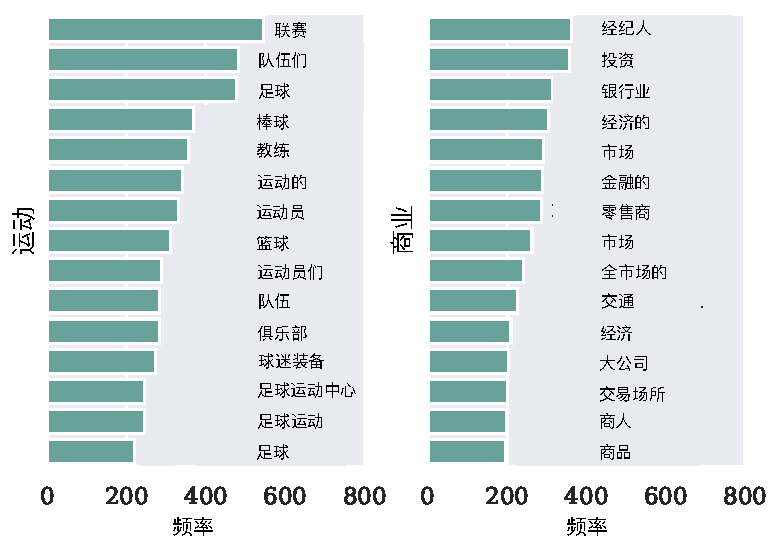
\includegraphics[width=\linewidth]{kptplots/toplabelwords_crop.zh.pdf}
    \caption{出现在前5个预测中的高频词}
    \label{fig:violin}
\end{figure}


\label{app:analysis}
\begin{figure}
    \centering
    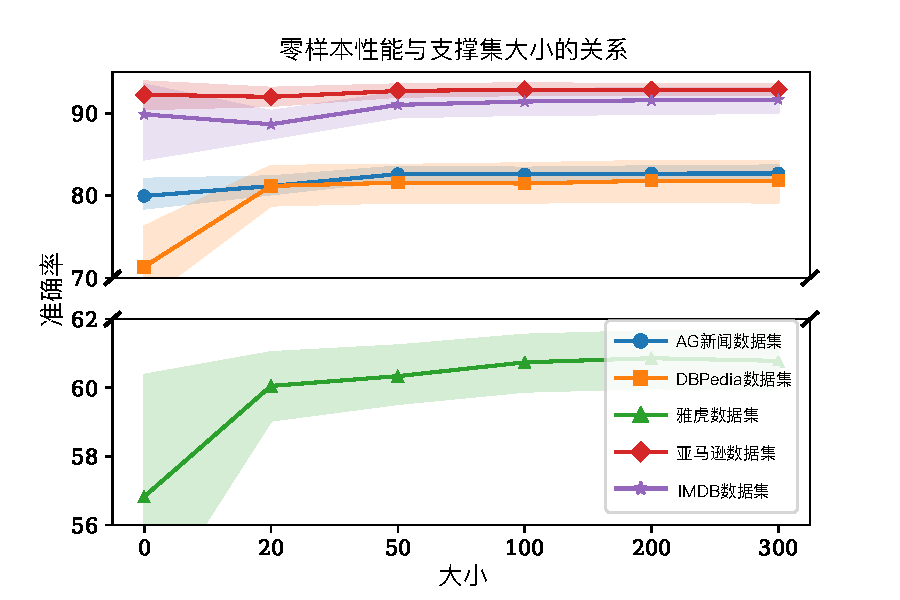
\includegraphics[width=\linewidth]{kptplots/SupportSetSize.zh.pdf}
    \caption{支持集大小与零样本性能的关系}
    \label{fig:calistudy}
\end{figure}

\subsubsection{校准与上下文校准}
\label{app:supportsize}
在微调中,校准已在预测置信度和分布外检测的研究中被探讨~\cite{kong-etal-2020-calibrated}。最近,它在提示学习中重新受到关注~\cite{pmlr-v139-zhao21c, holtzman2021surface}。在提示学习中,预训练语言模型倾向于预测某个词而忽略实际句子输入。例如,GPT-3在输入句子为“N/A”时更倾向于预测“positive”而非“negative”~\cite{pmlr-v139-zhao21c}。因此,在校准未进行后验优化时(即零样本学习中),校准至关重要(见表~\ref{tab:experiment-zero-shot})。现有方法如$\text{PMI}_\text{DC}$仅使用空模板而不填充语料库中的实例,例如“A \texttt{[Mask]} question :”,以生成校准对数。本文提出的上下文校准利用少量未标记的支持数据,显著提升了结果。然而,由于本文针对数据稀缺场景,详细研究了生成满意校准结果所需的未标记数据量。图~\ref{fig:calistudy}展示了KPT - RR在不同支持集大小$|\tilde{\mathcal{C}}|$下的性能,并与$|\tilde{\mathcal{C}}|=0$时的$\text{PMI}_\text{DC}$性能进行了对比。Size=0的点表示$\text{PMI}_\text{DC}$的性能。

从图~\ref{fig:calistudy}可以看出,$|\tilde{\mathcal{C}}|\sim 50$足以生成满意的校准结果。上下文校正在多类别分类中更为有效,而无上下文的校正在少类别分类中更为有效。

此外,必须指出的是,如果在实际场景中有一组句子需要分类,可以使用这些句子本身(因为校准集不需要标签)作为支持集进行更准确的上下文校准。

\subsubsection{监督数据减轻校准需求}
\label{app:fewshot-cali}
尽管校准在零样本设置中至关重要,但在少样本设置中本文未进行校准,因为假设标签词的后验概率可以通过少量训练实例调整到所需幅度。出于同样的假设,本文也未进行频率修正。为验证这一假设,本文在KPT中同时加入上下文校准和频率修正,并在不同设置下测试性能。结果如表~\ref{tab:experiment-fewshot-cc-rf}所示。绿色上箭头\gd 表示结果高于表~\ref{tab:experiment-few-shot}中的KPT,红色下箭头\bd 表示结果低于表~\ref{tab:experiment-few-shot}中的KPT。与表~\ref{tab:experiment-few-shot}中未使用CC和FR的KPT相比,性能对比通过上下箭头表示。可以看出,除了雅虎数据集数据集外,改进并不一致,甚至有时为负,这支持了本文的假设:监督输入数据大大减轻了校准的需求。

\begin{table}[!htbp]
\caption{少样本实验中的上下文校准和频率修正结果}
\begin{center}
\scalebox{0.70}{
\begin{tabular}{lllllll}
\toprule
样本数 & 方法  & AG新闻数据集   & DBPedia数据集 & 雅虎数据集 & 亚马逊数据集 & IMDB数据集  \\
\midrule
1 & KPT + CC + FR  & 83.4 \bd $\pm$ 4.0 \smallcolor{(84.6)} & 94.0 \gd $\pm$ 2.0 \smallcolor{(95.7)} & 63.3 \gd $\pm$ 2.0 \smallcolor{(64.9)} & 93.2 \nc $\pm$ 1.2 \smallcolor{(94.0)} & 92.1 \bd $\pm$ 3.2 \smallcolor{(93.8)} \\
5 & KPT + CC + FR  & 84.6 \bd $\pm$ 1.3 \smallcolor{(85.1)} & 97.3 \gd $\pm$ 0.3 \smallcolor{(97.4)} & 67.3 \gd $\pm$ 1.1 \smallcolor{(67.7)} & 94.0 \gd $\pm$ 1.2 \smallcolor{(94.7)} & 92.7 \nc $\pm$ 1.6 \smallcolor{(93.1)} \\
10 & KPT + CC + FR  &  85.9 \bd $\pm$ 1.7 \smallcolor{(86.7)} & 98.1 \gd $\pm$ 0.2 \smallcolor{(98.2)} & 68.0 \nc $\pm$ 1.1 \smallcolor{(68.6)} & 93.3 \bd $\pm$ 1.8 \smallcolor{(93.7)} & 92.9 \nc $\pm$ 1.8 \smallcolor{(93.6)} \\
20 & KPT + CC + FR  & 87.3 \gd $\pm$ 0.8 \smallcolor{(87.6)} & 98.0 \bd $\pm$ 0.4 \smallcolor{(98.2)} & 69.1 \gd $\pm$ 0.7 \smallcolor{(69.5)} & 93.5 \bd $\pm$ 1.1 \smallcolor{(93.9)} & 93.1 \nc $\pm$ 1.3 \smallcolor{(93.5)} \\
\bottomrule
\end{tabular}}
\end{center}
\label{tab:experiment-fewshot-cc-rf}
\end{table}

\begin{table}[!htbp]
\caption{限制扩展标签词为预训练模型词汇表中的单个标记的结果}
\begin{center}
\scalebox{0.70}{
\begin{tabular}{lllllll}
\toprule
样本数 & 方法  & AG新闻数据集   & DBPedia数据集 & 雅虎数据集 & 亚马逊数据集 & IMDB数据集  \\
\midrule
0 & KPT + ST & 84.9 \gd $\pm$ 1.0 \smallcolor{(86.3)} & 81.0 \bd $\pm$ 4.3 \smallcolor{(85.2)} & 62.7 \gd $\pm$ 1.1 \smallcolor{(64.4)} & 92.8 \nc $\pm$ 1.2 \smallcolor{(94.7)} & 91.5 \bd $\pm$ 2.8 \smallcolor{(94.1)} \\
1 & KPT + ST & 83.4 \bd $\pm$ 3.9 \smallcolor{(84.2)} & 94.0 \gd $\pm$ 1.8 \smallcolor{(95.8)} & 62.5 \bd $\pm$ 2.3 \smallcolor{(63.5)} & 93.3 \gd $\pm$ 1.4 \smallcolor{(94.1)} & 92.1 \bd $\pm$ 3.5 \smallcolor{(93.6)} \\
5 & KPT + ST & 84.7 \bd $\pm$ 1.8 \smallcolor{(85.4)} & 97.1 \nc $\pm$ 0.5 \smallcolor{(97.2)} &66.8 \bd $\pm$ 1.0 \smallcolor{(67.3)} & 93.3 \bd $\pm$ 2.1 \smallcolor{(93.8)} & 93.1 \gd $\pm$ 1.4 \smallcolor{(93.3)} \\
10 & KPT + ST & 86.3 \nc $\pm$ 1.5 \smallcolor{(86.8)} & 98.0 \nc $\pm$ 0.2 \smallcolor{(98.1)} & 67.6 \bd $\pm$ 0.9 \smallcolor{(67.9)} & 94.0  \gd $\pm$ 1.0 \smallcolor{(94.1)} & 92.7 \bd $\pm$ 1.8 \smallcolor{(93.6)} \\
20 & KPT + ST & 87.2 \bd $\pm$ 1.1 \smallcolor{(87.6)} & 97.9 \bd $\pm$ 0.4 \smallcolor{(98.1)} & 68.6 \bd $\pm$ 0.7 \smallcolor{(69.1)} & 93.5 \gd $\pm$ 1.8 \smallcolor{(94.0)} & 92.9 \bd $\pm$ 1.2 \smallcolor{(93.4)} \\
\bottomrule
\end{tabular}}
\end{center}
\label{tab:experiment-st}
\end{table}

\subsubsection{如何处理词汇表外的标签词?}
\label{app:experiment-st}
由于知识化标签词扩展使用的外部资源可能未针对预训练模型的词汇表进行定制,因此许多标签词是词汇表外的(OOV),并被分词器拆分为多个标记。对于这些词,如~\ref{sec:refine}所述,本文对每个标记在单个\texttt{[MASK]}位置上的预测概率进行平均,这在初看时可能不太合理。因此,本文进行了消融实验,研究是否强制标签词为预训练模型词汇表中的单个标记会带来更好的性能。不同shot下的结果如表~\ref{tab:experiment-st}所示。其中ST表示“单个标记”。绿色上箭头\gd 表示结果高于表~\ref{tab:experiment-few-shot}中的KPT,红色下箭头\bd 表示结果低于表~\ref{tab:experiment-few-shot}中的KPT。 令人惊讶的是,强制单标记限制并未带来稳定的改进,反而在许多情况下性能略有下降。因此,本文得出结论:处理被分词器拆分为多个标记的OOV标签词的方法是简单且合理的。更重要的是,通过知识库扩展但不在预训练模型词汇表中的标签词同样可以作为提示微调中的良好标签词。

\subsubsection{修正过程的可视化}
\label{app:remainwords}
本节报告了经过频率修正和相关性修正后剩余的标签词数量。从图~\ref{fig:remainwords}可以看出,这些修正方法去除了大部分标签词,同时保留了最具信息量的词。然而,即使剩余的标签词数量最少也超过100个,远多于之前工作中的标签词数量~\cite{schick2020automatically}。广泛的标签词覆盖是KPT成功的关键。

\begin{figure}[!htbp]
    \centering
    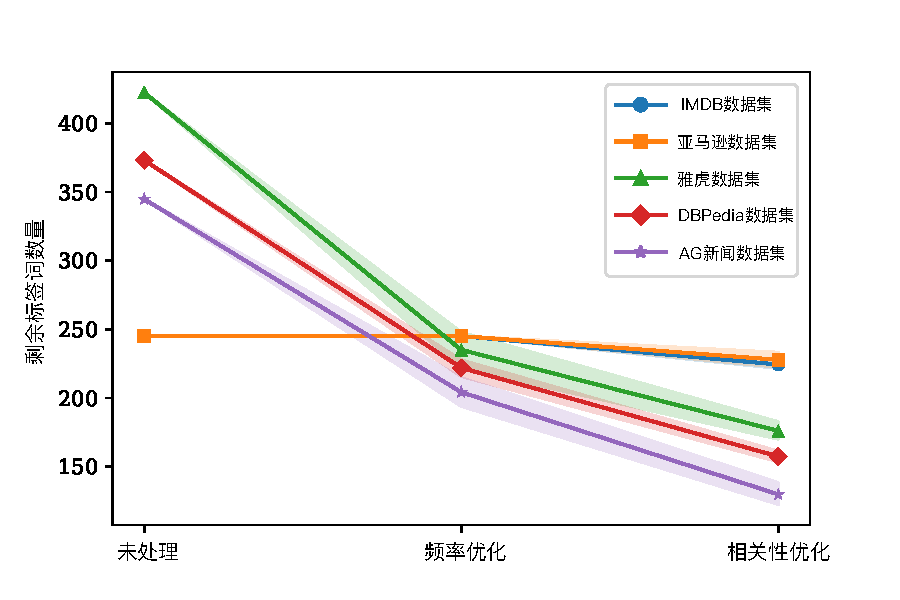
\includegraphics[width=0.96\linewidth]{kptplots/NRLW-3.zh.pdf}
    \caption{经过频率修正和相关性修正后剩余的标签词数量}
    \label{fig:remainwords}
\end{figure}

\subsubsection{无外部知识库的潜在使用}
\label{withoutkb}
尽管知识库在自然语言处理中无处不在,但在某些特定任务中可能没有现成的知识库可用。对于这些任务,如果有足够的未标记语料库,可以使用LOTClass~\cite{meng2020text}提出的方法从语料库中挖掘潜在的标签词。具体来说,LOTClass~\cite{meng2020text}使用自监督目标训练预训练模型,从整个未标记训练语料库中提取与主题相关的词。将KPT与LOTClass结合的实验超出了本文的范围,但本文相信两者的结合将非常有效。

\subsection{本章小结}


在本文中,我们研究了使用预训练语言模型来回答错误前提问题,这些问题对人类来说很简单,但却能欺骗大多数预训练语言模型。本文提出了第一个人工编写的错误前提问题数据集。通过使用该数据集,我们成功激活了预训练语言模型的区分和解释能力,并生成了既能回答通用问题又能稳健应对错误前提问题的预训练语言模型。对于未来的研究方向,我们认为可以将更先进的技术与 FalseQA 结合使用,以充分激活模型的能力,例如结合人类反馈的强化学习~\cite{ouyang2022training}。此外,将更多知识融入预训练语言模型也有助于其更好地回答错误前提问题。

在研究完能力激活方案后,本章进一步研究了知识激活方案。本章提出了KPT,该方法利用外部知识库扩展了提示微调中的标签词映射器。为了更好地利用知识库,本文提出了针对知识化标签词映射器的优化方法。实验表明,KPT在零样本和小样本设置中均展现出潜力。对于未来的工作,以下是与本研究相关的开放性问题值得探索:
1. 在模板构建和标签词映射器设计方面,结合知识库与提示微调的更好方法。
2. 将外部知识融入提示微调以应用于其他任务,如文本生成。

\improvement{这张和大题目结合不够紧需要改改}